\documentclass[finnish,twoside,censored,tkt,sw-line]{HYthesisML}


% In theses, open new chapters only at right page.
% For other types of documents, may ask "openany" in document.
\PassOptionsToClass{openright,twoside,a4paper}{report}
%\PassOptionsToClass{openany,twoside,a4paper}{report}

\usepackage{csquotes}
%%%%%%%%%%%%%%%%%%%%%%%%%%%%%%%%%%%%%%%%%%%%%%%%%%%%%%%%%
%% REFERENCES
%% Some notes on bibliography usage and options:
%% natbib -> you can use, e.g., \citep{} or \parencite{} for (Einstein, 1905); with APA \cite -> Einstein, 1905 without ()
%% maxcitenames=2 -> only 2 author names in text citations, if more -> et al. is used
%% maxbibnames=99 as no great need to suppress the biliography list in a thesis
%% for more information see biblatex package documentation, e.g., from https://ctan.org/pkg/biblatex

%% Reference style: select one
%% for APA = Harvard style = authoryear -> (Einstein, 1905) use:
% \usepackage[style=authoryear,bibstyle=authoryear,backend=biber,natbib=true,maxnames=99,maxcitenames=2,giveninits=true,uniquename=init]{biblatex}
%% for numeric = Vancouver style -> [1] use:
\usepackage[style=numeric,bibstyle=numeric,backend=biber,natbib=true,maxbibnames=99,giveninits=true,uniquename=init]{biblatex}
%% for alpahbetic -> [Ein05] use:
%\usepackage[style=alphabetic,bibstyle=alphabetic,backend=biber,natbib=true,maxbibnames=99,giveninits=true,uniquename=init]{biblatex}
%

\addbibresource{bibliography.bib}
% in case you want the final delimiter between authors & -> (Einstein & Zweistein, 1905)
% \renewcommand{\finalnamedelim}{ \& }
% List the authors in the Bibilipgraphy as Lastname F, Familyname G,
\DeclareNameAlias{sortname}{family-given}
% remove the punctuation between author names in Bibliography
%\renewcommand{\revsdnamepunct}{ }


%% Block of definitions for fonts and packages for picture management.
%% In some systems, the figure packages may not be happy together.
%% Choose the ones you need.

%\usepackage[utf8]{inputenc} % For UTF8 support, in some systems. Use UTF8 when saving your file.

\usepackage{lmodern}         % Font package, again in some systems.
\usepackage{textcomp}        % Package for special symbols
\usepackage[pdftex]{color, graphicx} % For pdf output and jpg/png graphics
\usepackage{epsfig}
\usepackage{subfigure}
\usepackage[pdftex, plainpages=false]{hyperref} % For hyperlinks and pdf metadata
\usepackage{fancyhdr}        % For nicer page headers
\usepackage{tikz}            % For making vector graphics (hard to learn but powerful)
%\usepackage{wrapfig}        % For nice text-wrapping figures (use at own discretion)
\usepackage{amsmath, amssymb} % For better math
\graphicspath{{../kuvat/}}

\singlespacing{}               %line spacing options; normally use single

\fussy
%\sloppy                      % sloppy and fussy commands can be used to avoid overlong text lines
% if you want to see which lines are too long or have too little stuff, comment out the following lines
% \overfullrule=1mm
% to see more info in the detailed log about under/overfull boxes...
% \showboxbreadth=50
% \showboxdepth=50



%%%%%%%%%%%%%%%%%%%%%%%%%%%%%%%%%%%%%%%%%%%%%%%%%%%%%%%%%
%% STEP 2:
%%%%%%%%%%%%%%%%%%%%%%%%%%%%%%%%%%%%%%%%%%%%%%%%%%%%%%%%%
%% Set up personal information for the title page and the abstract form.
%% Replace parameters with your information.
\title{Koneoppiminen lääkkeiden kehityksessä}

% TM: Contributors to template editors now listed in the beginning of the file in comments
\author{Heikki Pulli}
\date{\today}



% Set supervisors and examiners, use the titles according to the thesis language
% Prof.
% Dr. or in Finnish toht. or tri or FT, TkT, Ph.D. or in Swedish...
\supervisors{Leinonen, Matti}
\examiners{Prof.\ Ruotsalainen, Laura}


\keywords{Koneoppiminen, Lääkekehitys}
\additionalinformation{\translate{}}

%% For seminar reports:
%%\additionalinformation{Name of the seminar}

%% Replace classification terms with the ones that match your work. ACM
%% ACM Digital library provides a taxonomy and a tool for classification
%% in computer science. Use 1-3 paths, and use right arrows between the
%% about three levels in the path; each path requires a new line.

\classification{\protect{\ \ \
\  Computing Methodologies \(\rightarrow \) Machine Learning  \(\rightarrow \) Machine Learning Approaches \(\rightarrow \) Neural Networks, \\
\  Applied computing \(\rightarrow \) Life and medical sciences \(\rightarrow \) Health informatics
}}

%% if you want to quote someone special. You can comment this line out and there will be nothing on the document.
%\quoting{Bachelor's degrees make pretty good placemats if you get them laminated.}{Jeph Jacques}


%% OPTIONAL STEP: Set up properties and metadata for the pdf file that pdfLaTeX makes.
%% Your name, work title, and keywords are recommended.
% \hypersetup{
%     unicode=true,           % to show non-Latin characters in Acrobat’s bookmarks
%     pdftoolbar=true,        % show Acrobat’s toolbar?
%     pdfmenubar=true,        % show Acrobat’s menu?
%     pdffitwindow=false,     % window fit to page when opened
%     pdfstartview={FitH},    % fits the width of the page to the window
%     pdftitle={},            % title
%     pdfauthor={},           % author
%     pdfsubject={},          % subject of the document
%     pdfcreator={},          % creator of the document
%     pdfproducer={pdfLaTeX}, % producer of the document
%     pdfkeywords={something} {something else}, % list of keywords for
%     pdfnewwindow=true,      % links in new window
%     colorlinks=true,        % false: boxed links; true: colored links
%     linkcolor=black,        % color of internal links
%     citecolor=red,        % color of links to bibliography
%     filecolor=magenta,      % color of file links
%     urlcolor=cyan           % color of external links
% }

%%-----------------------------------------------------------------------------------

\begin{document}

% Generate title page.
\maketitle


%%%%%%%%%%%%%%%%%%%%%%%%%%%%%%%%%%%%%%%%%%%%%%%%%%%%%%%%%
%% STEP 3:
%%%%%%%%%%%%%%%%%%%%%%%%%%%%%%%%%%%%%%%%%%%%%%%%%%%%%%%%%
%% Write your abstract to be positioned here.
%% You can make several abstract pages (if you want it in different languages),
%% but you should also then redefine some of the above parameters in the proper
%% language as well, in between the abstract definitions.

\begin{abstract}

    Tässä tutkielmassa kerrotaan, kuinka koneoppimista voidaan käyttää lääkekehityksessä ja minkälaista dataa voidaan käyttää koneoppimismallien kouluttamisessa.
    Tutkielman alussa avataan nopeasti lääkekehityksen eri vaiheita ja miksi koneoppimista halutaan käyttää lääkekehityksessä.
    Seuraavissa kappaleissa keskitytään ainoastaan lääkkeiden löytämiseen ja lääkkeiden syntetisointisuunnitteluun ja kuinka koneoppimista voidaan hyödyntää näissä vaiheissa.
    Kappaleissa käydään läpi myös kolmen eri koneoppimismallin toimintaa, joista yksi keskittyy uusien lääkkeiden löytämiseen ja kaksi keskittyvät yhdisteiden syntetisointisuunnitteluun.
    Tutkielman alussa kerrotaan myös eri datatyypeistä, joita käytetään kyseisissä koneoppimismalleissa.

    Koneoppimismallien tarkoituksena on antaa lukijalle ajatus siitä, miten koneoppimista voidaan hyödyntää kyseisissä lääkekehityksen vaiheissa, minkälaisia ongelmia koneoppimismalleilla pyritään ratkomaan ja minkälaisia koneoppimismalleja ja tekniikoita ongelmien ratkomisessa on käytetty.


\end{abstract}

% \begin{otherlanguage}{english}
%     \begin{abstract}
%         Use this otherlanguage environment to write your abstract in another language if needed.

%         Topics are classified according to the ACM Computing Classification System
%         (CCS), see
%         \url{https://www.acm.org/about-acm/class}:
%         check command \verb+\classification{}+. A small set of paths (1--3) should be used, starting from any top nodes
%         referred to bu the root term CCS leading to the leaf nodes. The elements
%         in the path are separated by right arrow, and emphasis of each element individually can be indicated
%         by the use of bold face for high importance or italics for intermediate
%         level. The combination of individual boldface terms may give the reader
%         additional insight.
%     \end{abstract}
% \end{otherlanguage}

% Place ToC
\newpage
\mytableofcontents{}
\mainmatter{}

%%%%%%%%%%%%%%%%%%%%%%%%%%%%%%%%%%%%%%%%%%%%%%%%%%%%%%%%%
%% STEP 4: Write the thesis.
%%%%%%%%%%%%%%%%%%%%%%%%%%%%%%%%%%%%%%%%%%%%%%%%%%%%%%%%%
%% Your actual text starts here. You shouldn't mess with the code above the line except
%% to change the parameters. Removing the abstract and ToC commands will mess up stuff.
%%
%% You may wish to include material to avoid browsing the definitions
%% above. Command \include{file} includes the file of name file.tex.
%% As a side effect, subsequent inclusions may force a page break.

% BSc instructions
%\include{bsc_finnish_contents}
%\include{bsc_english_contents}
% MSc instructions
%\include{msc_finnish_contents}
% \include{msc_english_contents}

%%%%%%%%%%%%%%%%%%%%%%%%%%%%%%%%%%%%%%%%%%%%%%%%%%%%%%%%%

\chapter{Johdanto}

Uusien lääkkeiden kehittäminen on pitkä ja kallis prosessi.
Tähän kuuluu useita vaiheita ja eri vaiheet vievät eri määrän rahaa ja aikaa.
Vaiheet ovat sairauden aiheuttajan tunnistaminen, aiheuttajaan vaikuttavan lääkkeen tunnistaminen, lääkkeen optimointi, lääkkeen ominaisuuksien analysointi ja kliiniset testit.
Näiden vaiheiden jälkeen lääke joko hyväksytään myyntiin tai sitä joudutaan edelleen jatkokehittämään.
Kaikki vaiheet yhdessä ovat tavallisesti vieneet 10--12 vuotta ja niiden hinnaksi on voinut muodostua 1--3 miljardia dollaria~\cite{EkinsSean2019Emlf}.

Vaiheiden pitkän keston ja korkean hinnan takia tutkijat ja lääkealan yritykset ovat alkaneet tutkia uusia keinoja, jotka nopeuttaisivat lääkkeiden tutkimista tai laskisivat lääkekehityksen prosessin hintaa.
Koneoppimismallit ovat nousseet houkuttelevaksi vaihtoehdoksi ratkaisemaan näitä ongelmia.
Yritykset ovat alkaneet selvittää, kuinka eri koneoppimismalleja voidaan käyttää lääketutkimuksen suurimpien pullonkaulojen poistamiseksi~\cite{EkinsSean2019Emlf}.

Viimeisen kymmenen vuoden aikana saatavilla olevan laadukkaan datan määrä on kasvanut merkittävästi ja samalla on kehitetty uusia ja tehokkaampia koneoppimismalleja, joita voidaan hyödyntää lääketutkimuksessa~\cite{ButlerKeithT2018Mlfm,VamathevanJessica2019Aoml}.
Koneoppimismallien avulla voidaan esimerkiksi karsia kaikista harkinnassa olevista lääkkeistä lupaavimmat kandidaatit, joilla on mahdollisuus päästä testeistä läpi tuotantoon asti~\cite{GayvertKaitlyn}.
Koneoppimismalleja voidaan myös hyödyntää aivan uusien lääkkeeksi sopivien yhdisteiden etsimisessä~\cite{ShinBonggun,ShaharHarelAndKiraRadinsky}.
Tähän tarkoitukseen kehitetyt koneoppimismallit kykenevät etsimään lääkkeitä, joilla on halutut lääkkeelliset ja fysikaaliset ominaisuudet~\cite{VamathevanJessica2019Aoml}.
Kehitetyt mallit ovat näyttäneet, että koneoppimismallit ovat tehokkaita työkaluja, joita voidaan hyödyntää kaikissa lääketutkimuksen eri vaiheissa.

Tässä tutkielmassa paneudutaan muutamiin koneoppimismalleihin, joita käytetään uusien lääkkeiden tunnistamisessa ja näiden tunnistettujen lääkkeiden syntetisointisuunnittelussa.
Tutkielman tarkoituksena on tutustuttaa lukija koneoppimisen käsitteistöön ja erilaisiin malleihin ja ongelmiin, jotka liittyvät lääkkeiden löytämiseen ja löydettyjen lääkkeiden syntetisointisuunnitteluun.
Käsiteltävät koneoppimismenetelmät toimivat esimerkkeinä, kuinka koneoppimista voidaan käyttää käsiteltävissä konteksteissa.

Ensimmäisessä kappaleessa tutustutaan eri datatyyppeihin, joita käytetään koneoppimismallien kouluttamisessa.
Tämä on lyhyt kappale, jossa käydään läpi ne datatyypit, joita myöhemmin selitettävät koneoppimismallit käyttävät.
Datatyyppien ymmärtäminen auttaa hahmottamaan myöhemmin tutkielmassa selitettävien eri mallien toimintaperiaatteita.

Toisessa kappaleessa käydään läpi, kuinka uusia lääkkeitä etsitään ja löydetään.
Kappaleessa avataan pintapuolisesti läpi virtuaalista seulontaa (Virtual Screening), mitä sillä tarkoitetaan ja kuinka sitä hyödynnetään.
Tässä kappaleessa käydään läpi myös yhden koneoopimismallin toimintaa, joka on koulutettu löytämään uusia yhdisteitä.
Tämä malli mahdollistaa uusien lääkeyhdisteiden nopean löytämisen, joita päästään jatkotutkimaan nopeasti.

Kolmas kappale paneutuu yhdisteiden syntetisointiin ja kuinka sitä voidaan toteuttaa hyödyntämällä koneoppimismalleja.
Kappaleessa käsitellään, kuinka syntetisointia voidaan suunnitella retrosynteesianalyysin avulla, mikä tekee yhdisteiden retrosyntetisointianalyysista hankalaa ja mitä ratkaisuja tähän on kehitetty.
Kappale kertoo CASP-menetelmistä (Computer Aided Synthesis Planning) ja kuinka tämä liittyy retrosyntetisointianalyysiin.
Kappaleessa avataan myös kahden eri koneoppimismallin toimintaa, jotka on kehitetty auttamaan eri yhdisteiden syntetisointisuunnittelussa.

\chapter{Kemiallinen data}

Tässä kappaleessa kerrotaan pintapuolisesti, minkälaista dataa käytetään koneppimismallien kouluttamisessa.
Kappaleessa keskitytään datatyyppeihin, joita käytetään koneoppimismalleissa, joiden toimintaa tullaan avaamaan tämän tutkielman muissa osissa.
Koneoppimismallit, joiden toimintaa avataan, käyttävät datatyyppejä, joilla kuvataan pienyhdisteitä.
Tämän takia kappaleessa keskitytään vain pienyhdisteitä kuvaaviin datatyyppeihin.
Kappaleessa käydään läpi SMILES- ja SMARTS-datatyypit, mihin niitä käytetään ja kuinka ne eroavat toisistaan.
Kappaleessa myös kerrotaan, mitä ovat yhdisteiden ECFP-tunnisteet, mitä ominaisuusvektorit ovat ja mitä tietoa ne sisältävät yhdisteistä.

\section{Yhdisteiden kuvaaminen merkkijonoilla}

Tavallinen tapa kuvata yhdisteitä on kuvata ne yhdellä rivillä merkkijonona.
SMILES (Simplified Molecular Input Line Entry System) on David Weiningerin vuonna 1988 kehittämä tapa kuvata molekyylejä ja yksinkertaisia yhdisteitä~\cite{WeiningerSMILES}.
Se kuvaa yhdisteen yhdellä rivillä käyttäen ASCII-merkistöä.
Tämän takia se on tietokoneen nopea lukea ja kemistin helppo ymmärtää.
Kuvassa~\ref{fig:melatonin} on esitetty melatoniiniyhdiste ja kuinka se kuvataan SMILES-standardin mukaisesti.

\begin{figure}[!ht]
    \centering
    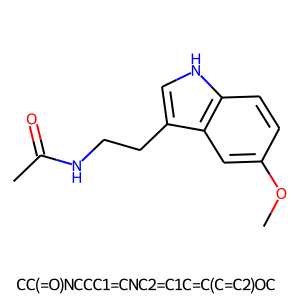
\includegraphics[width=6cm, height=6cm]{melatonin-smiles.png}
    \caption{Melatoniiniyhdiste, kuinka se kuvataan graaffina ja SMILES-merkijonona.
        Kuva on tuotettu hyödyntämällä RDKit-kirjastoa.}
    {\label{fig:melatonin}}
\end{figure}

SMARTS (SMILES Arbitrary Target Specification) on SMILES-standardista jatkokehitetty tapa kuvata yhdisteitä.
Se mahdollistaa yhdisteiden sisäisten rakenteiden määrittämisen.
SMARTS on yläluokka SMILES-standardista, jonka takia kaikki SMILES-merkkijonoiksi kelpaavat merkkijonot ovat myös kelpoja SMARTS-merkkijonoja.
SMARTS- ja SMILES-standardit mahdollistavat myös kemiallisten reaktioiden kuvaamisen ASCII-merkistöllä yhdellä rivillä.

\section{Yhdisteiden kuvaaminen bitteinä, ECFP}

Toinen tavallinen tapa kuvata yhdisteitä on muuttaa ne ECFP (Extended Connectivity Fingerprint) bittijonoiksi~\cite{RogersDavid2010EF}.
ECFP-tunniste lasketaan käyttämällä Morganin algoritmia.
Algoritmi laskee jokaiselle yhdisteen atomille numeerisen arvon käyttämällä hajautusfunktiota ja iteroimalla ja laskemalla näitä arvoja yhteen se saa laskettua yhdisteen eri osille niitä kuvaavat numeeriset arvot.
ECFP-tunnisteita kutsutaan myös Morgan-tunnisteiksi (Morgan Fingerprint).
Nämä numeeriset arvot voidaan muuttaa sitten halutun mittaisiksi bittiesityksiksi~\cite{RogersDavid2010EF}.
ECFP on yksi monista tavoista kuvata yhdisteitä numeerisessa muodossa, mutta se on yksi käytetyimmistä menetelmistä sen nopean ja helpon laskemisen takia.
Bittijonojen etuna on se, että lyhyet bittijonot vievät vähän muistia, mutta lyhyiden bittijonojen ongelmana on, että ne saattavat menettää oleellista tietoa yhdisteestä bittitörmäysten takia.
Tämän takia tavallisesti käytetään 4096-bitin mittaisia bittijonoja.

\section{Ominaisuusvektorit}

Yksi tässä tutkielmassa käsiteltävistä koneoppimismalleista käyttää ominaisuusvektoreita hyödykseen.
Ominaisuusvektorit sisältävät tietoa yhdisteen tai molekyylin lääkkeellisistä ominaisuuksista.
Ominaisuusvektorit voivat kuvata mitä tahansa yhdisteen tai molekyylin ominaisuutta ja ne voidaan valita tilanteen mukaan.
Kyseisessä mallissa ominaisuusvektorit kuvaavat molekyylin PlogP, QED ja DRD2 arvoja~\cite{ShinBonggun}.
PlogP (Penalized LogP) kuvaa aineen rasvaliukoisuutta, QED (Quantitative Estimate of Drug-likeness) kuvaa tietyn yhdisteen lääkkeenkaltaisuutta ja DRD2 kuvaa, kuinka paljon molekyyli reagoi dopamiini 2 reseptoria vastaan~\cite{BickertonGRichard2012Qtcb}.
Nämä ovat oleellisia tietoja tutkittaessa uusia mahdollisia lääkeyhdisteitä~\cite{ShinBonggun}.

\chapter{Uusien lääkkeiden löytäminen}

Tässä kappaleessa kerrotaan, mitä asioita liittyy lääkkeiden löytämiseen.
Kappaleessa avataan, mitä on virtuaalinen seulonta ja kuinka sitä hyödynnetään lääkkeiden etsinnässä.
Kappaleessa avataan myös yhden koneoppimismallin toimintaperiaate.
Kyseinen koneoppimismalli luo uusia lääkkeitä kuvaavia SMARTS-merkkijonoja, joilla on mahdollisimman lähellä haluttuja ominaisuuksia olevat ominaisuudet.

\section{Lääkkeiden löytäminen}

Yksi ensimmäisistä lääkekehityksen osa-alueista on uusien lääkkeiksi kelpaavien yhdisteiden löytäminen joko uusiin tai jo tunnettuihin tauteihin~\cite{EkinsSean2019Emlf}.
Lääkeyhdisteiden löytäminen on kuitenkin ollut tavallisesti hidas prosessi ja uuden toimivan yhdisteen löytäminen on kestänyt useita vuosia~\cite{EkinsSean2019Emlf,MunosBernardH2011Htrb}.
On itse asiassa huomattu, että uusien lääkkeiden löytäminen on muuttunut yhä kalliimaksi ja uusia lääkkeitä tulee markkinoille vähemmän kuin aikaisemmin~\cite{MunosBernardH2011Htrb}.
Koneoppimista on alettu hyödyntämään tässä vaiheessa prosessiin kuluvan ajan nopeuttamiseksi~\cite{VamathevanJessica2019Aoml}.

Viimeisen kymmenen vuoden aikana saatavilla olevan datan määrä koskien lääkkeitä ja lääkeyhdisteitä on kasvannut merkittävästi kehitettyjen tietopankkien ansiosta~\cite{EkinsSean2019Emlf}.
Tietopankkeja ovat esimerkiksi PubChem ja ChEMBL~\cite{NationalCenterForBiotechnologyInformation,chembl}.
Molemmat näistä keskittyvät lääkeyhdisteiden tietojen tallentamiseen.
PubChem on Yhdysvaltojen terveysviraston (National Institute of Health) ylläpitämä ja ChEMBL on Euroopan bioinformatiikka instituution (European Bioinformatics Institute, EBI) ylläpitämä.

\section{Virtuaalinen seulonta}

Kemiallisten yhdisteiden avaruudella tarkoitetaan kaikkien uniikkien yhdisteiden lukumäärää.
On arvioitu, että erilaisia kemiallisia yhdisteitä, jotka voivat esiintyä huoneenlämmössä nesteessä, voi olla välillä \(10^{18} - 10^{180}\)~\cite{SotrifferChristoph2011VSPC}.
Yhdisteet, jotka täyttävät lääkkeeltä vaaditut kriteerit, on puolestaan arvioitu olevan noin \(10^{60}\)~\cite{SotrifferChristoph2011VSPC}.
Erillaisten yhdisteiden suuri lukumäärä itsessään esittää tarpeen tehokkaille algoritmeille ja menetelmille, jotka auttavat karsimaan tästä suuresta määrästä kemiallisia yhdisteitä vain lupaavimmat.

Virtuaalinen seulonta (Virtual Screening) on suosittu lähestymistapa uusien lääkkeiden tai lääkkeeksi kelpaavien yhdisteiden löytämiseksi.
Virtuaalinen seulonta käsittää joukon menetelmiä, joissa tietokoneita hyväksi käyttäen karsitaan yhdisteiden avaruudesta vain tietyt kriteerit täyttävät yhdisteet~\cite{SotrifferChristoph2011VSPC}.
Yhdisteiden karsimisessa käytetään ohjelmistoja, joissa toteutetut algoritmit suorittavat seulontaa annettujen parametrien avulla.

Koneoppimismenetelmiä voidaan myös käyttää virtuaalisessa seulonnassa~\cite{SotrifferChristoph2011VSPC}.
Yleisimpiä koneoppimismenetelmiä ovat tällä hetkellä SVM (Support Vector Machine) ja Random forest -mallit~\cite{SotrifferChristoph2011VSPC}.
Neuroverkko ja Ensemble-koneoppimismallit ovat myös yleistyneet viimevuosina~\cite{ShinBonggun,PopovaMariya2018Drlf}.
Ensemble-mallien ideana on yhdistää useita eri koneoppimismalleja yhdeksi malliksi~\cite{RokachLior2009Ec}.
Ensemble-mallit ovat tavallisesti parempia ja monipuolisempia toiminnalisuuksissaan kuin yksittäiset koneoppimismallit ja ne myös tuottavat tarkempia tuloksia.
Koneoppimismallien avulla löydettyjä yhdisteitä voidaan jatkotutkia ja kehittää edelleen lääkkeiksi.

\section{Kehitettyjä koneoppimismalleja}

Seuraavaksi avataan erään toteutetun koneoppimismallin toimintaperiaatetta.
Kyseinen malli etsii uusia lääkkeitä käyttämällä hyödyksi sille annettua prototyyppiyhdistettä, prototyypin kemiallisia ominaisuuksia ja uudelta lääkkeeltä haluttuja kemiallisia ominaisuuksia.
Kemialliset ominaisuudet on koodattu ominaisuusvektoreihin.

\subsection{CMG-malli}

CMG (Controlled Molecule Generator) on koneoppimismalli, joka etsii uusia molekyylejä, jotka perustuvat syötteenä annettuun molekyyliin ja joilla on ennalta määritellyt halutut ominaisuudet~\cite{ShinBonggun}.
CMG-mallin toimintaperiaatteena on muokata prototyyppiyhdistettä siten, että se maksimoi halutut ominaisuudet, jotka on määritelty sen syötteenä saamassa ominaisuusvektorissa.
CMG-mallin toimintaa rajoittaa kuitenkin prototyyppiyhdiste ja syötteenä annettu samanlaisuusluku, jonka alle uuden luodun yhdisteen ja prototyyppiyhdisteen välinen tanimoto-indeksi ei saa mennä.
Tanimoto-indeksi kuvaa, kuinka paljon molekyylit muistuttavat toisiaan rakenteellisesti~\cite{MaggioraGerald2014Msim}.
Tanimoto-indeksin arvot ovat välillä \([0,1]\).

CMG-malli eroaa aikaisemmin kehitetyistä malleista siten, että se pystyy optimoimaan annetun molekyylin useampaa ominaisuutta samanaikaisesti.
Aikaisemmin kehitetyt mallit ovat pystyneet optimoimaan vain yhtä molekyylin ominaisuutta.

CMG-malli muodostuu kolmesta verkosta, joista kaksi verkkoa toimivat rajoiteverkkoina.
Ensimmäinen verkko on MTN (Molecule Translation Network) ja rajoiteverkot ovat PPN (Property Prediction Network) ja SPN (Similarity Prediction Network).
Kuvassa~\ref{fig:cmg-model-whole} näkyy CMG-mallin rakenne ja toimintaperiaate.

CMG-mallin kehittäjät lähestyvät molekyylin ominaisuuksien optimointiongelmaa merkkijonojen käännös- ja luontiongelmana.
CMG-mallille opetetaan, kuinka syötteenä annettu yhdistemerkkijono käännetään sellaiseksi yhdistemerkkijonoksi, jolla on lähimpänä haluttuja ominaisuuksia olevat ominaisuudet.
CMG-malli tulkitsee ensin annetut merkkijonot hyödyntäen DN-verkkoa (Deep Network) jonka jälkeen se luo uusia molekyyliyhdisteitä hyödyntäen tätä tulkintaa ja haluttua ominaisuusvektoria.
Koska ominaisuudet annetaan vektorina, niin CMG-malli pystyy optimoimaan useampaa ominaisuutta samanaikaisesti.
CMG-malli hyödyntää myös etukäteen koulutettuja rajoiteverkkoja (Constraint Network), jolloin vältytään luomasta mahdottomia yhdisteitä.
CMG-malli käyttää näitä verkkoja hyödyksi muokattussa Beam Search -algoritmissa.

Beam Searh -algoritmi saa syötteenä kaikki CMG-mallin kehittämät yhdisteet, pisteyttää ne ja palauttaa yhdisteen, joka sai parhaimman pisteytyksen.
Algoritmi käyttää PPN-verkkoa ennustaessaan kehitetyn molekyylin ominaisuuksia ja SPN-verkkoa laskiessaan, kuinka samankaltainen kehitetty yhdiste on CMG-mallin syötteenä saadun yhdisteen kanssa.
Näiden tietojen avulla algoritmi laskee kehitetyille yhdisteille numeeriset arvot ja palauttaa yhdisteen, joka saa parhaimman arvon.

Data, jolla mallit koulutetaan, on peräisin ZINC-tietokannasta ja DRD2-dataseteistä.
ZINC on ilmainen tietokanta, joka sisältää tietoa lääkeyhdsteistä, ja jota voidaan käyttää virtuaalisessa seulonnassa~\cite{ZINC}.
ZINC tietokantaa ylläpitää Irwin ja Shoichet laboratoriot Kalifornian yliopistossa.
DRD2-datasetti sisältää tietoa yhdisteistä ja kuinka nämä yhdisteet reagoivat dopamiini 2 reseptorin kanssa.
DRD2-datasetti luotiin Olivecrona et al.\ tutkimuksen yhteydessä ja sitä käytetään samalla tavalla CMG-mallissa~\cite{ShinBonggun}.

Data sisältää kaiken kaikkiaan 257 565 molekyyliä, joista luodaan pareja.
Parit muodostetaan siten, että kahden molekyylin välinen tanimoto-indeksi on yli 0.4.
Näitä \((X,Y)\) pareja muodostetaan kaiken kaikkiaan 10 827 615 kappaletta.
Lisäksi kaikille molekyyleille lasketaan niiden eri kemiallisten ominaisuuksien arvot, jotka ovat PlogP, QED ja DRD2.
Nämä kuvaavat eri ominaisuuksia, joita malli pyrkii optimoimaan halutulla tavalla.

\begin{figure}[!ht]
    \centering
    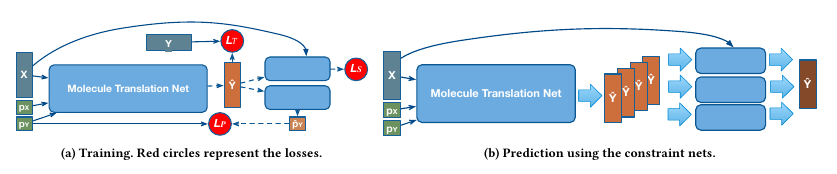
\includegraphics[width=\textwidth]{CMG-fig.png}
    \caption{CMG-mallin toimintaperiaate kuvattuna}
    {\cite{ShinBonggun}}
    {\label{fig:cmg-model-whole}}
\end{figure}

\subsubsection{MTN-verkko}

MTN-verkko perustuu aikaisemmin kehitettyyn The Transformer -malliin~\cite{TheTransformer}.
The Transformer -malli eroaa aikaisemmin yleisistä NLP-malleista siten, että se perustuu täysin attention-perusteiseen lähestymistapaan.
The Transformer -malli noudattaa encoder-decoder arkkitehtuuria.
Encoder-osio muuntaa ensin saamansa syötteen jokaisen sanan todennäköisyysjakaumaksi ja nämä todennäköisyysjakaumat syötetään decoder-osiolle.
Tämän todennäköisyysjakauman ja aikaisemman sanan avulla se määrittää seuraavan sanan tulosteeseen.

MTN-verkko eroaa The Transformer -mallista kahdella tavalla.
Toisin kuin The Transformer -malli, joka käsittelee sanoja ja niistä muodostettuja lauseita, MTN-verkko käsittelee yksittäisiä merkkejä ja niistä muodostettuja molekyylejä.
Lisäksi MTN-verkon piilotettuun tasoon on lisätty tietoa kemiallisista ominaisuuksista.

\subsubsection{PPN-verkko}

PPN-verkon rakenne ja toiminta periaate näkyvät kuvassa~\ref{fig:cmg-model-ppn}.
PPN-verkko ottaa syötteenä ennustetun molekyylin merkkijonon (\(y_i\)).
Tämä merkkijono muunnetaan piilotetuiksi vektoreiksi hyödyntäen Bidirectional Long Short-Term Memory (BiLSTM) -tasoa.
BiLSTM-taso on rakenteeltaan samanlainen kuin LSTM-taso, mutta koska se käsittelee syötteen sekä alku-loppu suunnassa että loppu-alku suunnassa se oppii tietyn merkin kontekstin molemmissa suunnissa.
BiLSTM-taso muodostaa vektoreita oikealta vasemmalle ja vasemmalta oikealle suunnissa.
Näistä vektoreista valitaan molempien suuntien viimeiset vektorit.
Nämä vektorit yhdistetään ja yhdistevektori syötetään täysin yhdistetylle neuroverkolle.
Tämä verkko sisältää kaksi piilotettua tasoa.
Verkko antaa tuloksena kyseisen yhdisteen ominaisuuksien ennusteen.

PPN-verkko koulutetaan käyttäen 257 565 eri molekyyliä.
Nämä molekyylit jaetaan sattumanvaraisella valinnalla koulutus- ja testiryhmiin suhteessa 8:2.

\subsubsection{SPN-verkko}

SPN-verkon rakenne ja toimintaperiaate on kuvattu kuvassa~\ref{fig:cmg-model-spn}.
SPN-verkko ottaa syötteenä ennustetun molekyylin merkkijonon (\(y_i\)) ja alkuperäisen molekyylin merkkijonon (\(x_i\)).
Nämä merkkijonot syötetään kahdelle eri biLSTM-tasolle, toinen käsittelee alkuperäisen molekyylin merkkijonot ja toinen ennustetun molekyylin merkkijonot.
Nämä biLSTM-tasot tomivat samalla periaatteella kuin PPN-verkossa ja palauttavat näin ollen neljä eri vektoria, kaksi ennustetulta merkkijonolta ja kaksi alkuperäiseltä merkkijonolta.
Nämä vektorit yhdistetään ja tämä yhdistevektori annetaan täysin yhdistetylle verkolle, joka sisältää kaksi piilotettua tasoa.
Tämä verkko toimii binääriluokittelijana ja palauttaa tiedon, onko kaksi syötemolekyyliä samanlaisia määritellyn samanlaisuusrajan mukaan.

SPN-verkon kouluttamiseen käytetään osajoukkoa 10 827 615 eri parista.
Tästä määrästä valitaan kymmenen prosentin osajoukko, joka on 997 773 molekyylin suuruinen.
Tämä joukko jaetaan samalla tavalla koulutus- ja testiryhmiin kuin PPN-verkossa.

\begin{figure}[!ht]
    \centering
    \begin{minipage}[b]{0.4\textwidth}
        \centering
        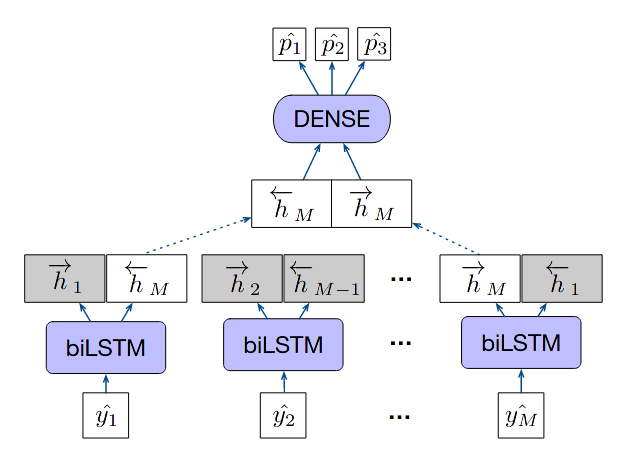
\includegraphics[width=\textwidth]{cmg-property-prediction-network.png}
        \caption{PPN-verkon rakenne}
        {\cite{ShinBonggun}}
        {\label{fig:cmg-model-ppn}}
    \end{minipage}
    \hfill
    \begin{minipage}[b]{0.4\textwidth}
        \centering
        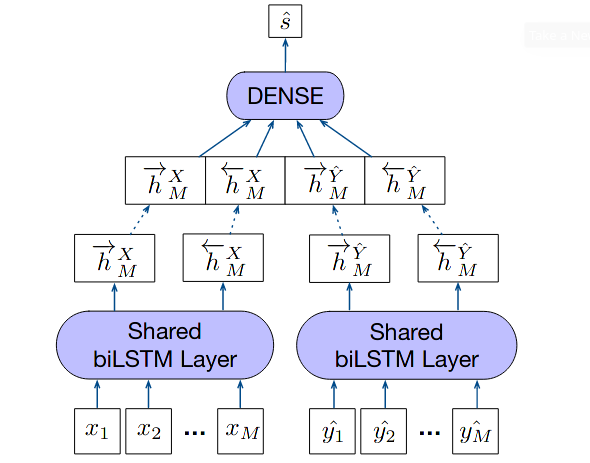
\includegraphics[width=\textwidth]{cmg-similarity-network.png}
        \caption{SPN-verkon rakenne}
        {\cite{ShinBonggun}}
        {\label{fig:cmg-model-spn}}
    \end{minipage}
\end{figure}

\chapter{Uusien lääkkeiden syntetisointi}

Tässä kappaleessa kerrotaan, miten lääkkeiden syntetisointisuunnittelua voidaan tehostaa koneoppimismallien avulla.
Kappaleessa keskitytään syntetisointisuunnitteluun retrosyntetisointimenetelmää hyödyntämällä.
Kappaleessa kerrotaan, mikä tekee yhdisteen retrosyntetisoinnista vaikeaa ja kuinka sitä voidaan tehostaa hyödyntämällä eri koneoppimismalleja.
Kappaleessa avataan kahden koneoppimismallin toimintaa, jotka suorittavat halutun yhdisteen retrosyntetisointia.

\section{Yhdisteiden syntetisointi}

Yhdisteen syntetisointisuunnittelulla tarkoitetaan prosessia, jossa määritellään, kuinka haluttu yhdiste voidaan tuottaa synteettisesti saatavilla olevista lähtöaineista~\cite{ColeyConnorW2018MLiC}.
Retrosynteesianalyysillä tarkoitetaan puolestaan menetelmää, jonka avulla löydetään halutun yhdisteen tuottamiseen tarvittavat lähtöaineet.
Retrosynteesianalyysi toimii siis toiseen suuntaan kuin syntetisointi.
Retrosynteesissä yhdiste pilkotaan rekursiivisesti pienempiin lähtöaineisiin kunnes jäljellä on vain saatavilla olevia lähtöaineita~\cite{ECoreyRetrosynthesis}.

Tavallisesti yhdisteen retrosyntetisointi on vaatinut suorittavalta kemistiltä usean vuoden kokemusta ja tietoa saatavilla olevista lähtöaineista ja eri reaktioista.
Retrosyntetisointia on pyritty automatisoimaan eri CASP-menetelmien avulla (Computer-Aided Synthesis Planning).
CASP on jo 1960-luvulla kehitetty ajatus, ja ensimmäisiä yrityksiä toteuttaa retrosyntetisointia tekoälyn avulla oli E.J Coreyn LHASA-projekti~\cite{ColeyConnorW2018MLiC}.
LHASA perustui heuristisiin algoritmeihin, joissa kemistit käsin koodasivat, miten eri lähtöaineet reagoivat keskenään ja mikä on reaktion lopputuote~\cite{LHASA}.
Tämä on kuitenkin osoittautunut toivottomaksi yritykseksi valtavan datamäärän takia.

Kehitys koneoppimismenetelmissä on kuitenkin tarjonnut uuden lähestymistavan CASP-menetelmien kehityksessä.
Sen sijaan, että kemistit kehittäisivät heuristisia malleja, uudet koneoppimismallit koulutetaan saatavilla olevan datan avulla.
Tämä on todettu merkittävästi paremmaksi lähestymistavaksi~\cite{ColeyConnorW2018MLiC}.

Koneoppimismallien käyttö ja koulutus ei ole kuitenkaan täysin ongelmaton lähestymistapa.
Ongelmaan liittyvää dataa ei välttämättä ole saatavilla ja datan hankkiminen voi olla kallista~\cite{deAlmeidaA.Filipa2019Socd}.
Vielä ei ole kehitetty julkista ja kaikille avointa tietopankkia, joka sisältäisi tietoa kemiallisista reaktioista, vaan ainoastaan kaupallisia tietopankkeja on kehitetty, kuten Reaxys ja SciFinder~\cite{deAlmeidaA.Filipa2019Socd}.

\section{Lääkkeen retrosyntetisoinnin haastavuus}

Retrosyntetisoinnin tekee hankalaksi se, että tutkittaessa kuinka haluttu yhdiste voidaan muodostaa, tulee käydä läpi satojatuhansia mahdollisia kemiallisia muunnoksia, joiden avulla voidaan luoda haluttu yhdiste~\cite{SeglerMarwinHS2018Pcsw}.
Kemiallisella muunnoksella tai myöhemmin käytetyllä termillä muunnossääntö tarkoitetaan yleisesti kaikkia mahdollisia reaktioita tai reaktiotyyppejä, joita kemiassa tunnetaan.
Tämä ongelma toistuu rekursiivisesti, kun yhdiste pilkotaan yhdisteisiin, jotka keskenään reagoidessaan muodostavat alkuperäisen yhdisteen.
Kuvassa~\ref{fig:retrosynthesis-example} näkyy, kuinka monella tavalla yksinkertainen yhdiste voidaan muodostaa.
Pienille ja yksinkertaisille yhdisteille tämä muunnostenavaruus on pienempi, mutta yhdisteen koon kasvaessa eri tapojen määrä muodostaa haluttu yhdiste kasvaa eksponentiaalisesti.
Tästä johtuen tarve prosessia yleistäville koneoppimismalleille on iso.

\begin{figure}[!ht]
    \centering
    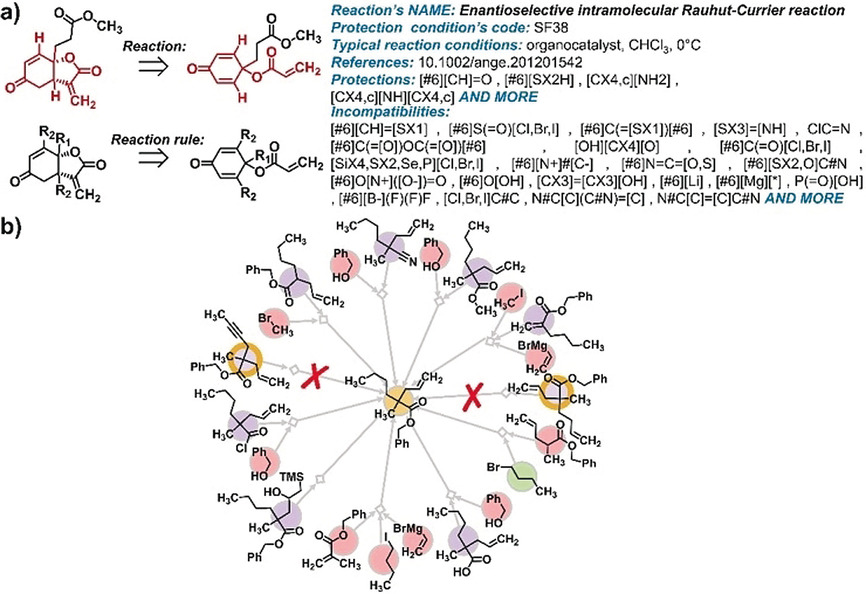
\includegraphics[width=\textwidth]{retrosynthesis.jpg}
    \caption{(a) esimerkki reaktiosäännöstä, (b) esimerkki mahdollisista reaktioista, kuinka voidaan luoda haluttu yhdiste (keskellä).
        Kuvaa on yksinkertaistettu ja se sisältää vain yksitoista mahdollista reaktiota, jotka tuottavat halutun yhdisteen.
        Värikoodaukset tarkoittavat: keltainen --- haluttu yhdiste, punainen --- saatavilla oleva yhdiste, vihreä --- kirjallisuudesta tunnettu yhdiste, liila --- tuntematon yhdiste}
    {\cite{ExpertKnowledgeRetorsynthesis}}
    {\label{fig:retrosynthesis-example}}
\end{figure}


\section{Kehitettyjä apuvälineitä}

Seuraavissa luvuissa avataan kahden kehitetyn koneoppimismallin toimintaa.
Nämä mallit on toteutettu suorittaman retrosynteesianalyysiä, mutta niiden toimintaperiaate perustuu eri lähestymistapoihin.

3N-MCTS-malli on kokonaisempi malli, koska se palauttaa retrosyntetisointipolun, joka kertoo, kuinka haluttu yhdiste voidaan syntetisoida laboratoriossa.
Se suodattaa jokaisessa retrosyntetisointivaiheessa kaikista mahdollisista muunnoksissta vain ne, jotka ovat toteutettavissa.
Monte Carlo -puuhakualgoritmi etsii näiden suodatettujen muunnosten avulla retrosyntetisointipolun.

ICHO-malli palauttaa parhaan muunnossäännön, jonka avulla haluttu yhdiste voidaan muodostaa.
ICHO-mallin toiminta on verrattavissa 3N-MCTS-mallissa käytetettyihin koneoppimismalleihin, jotka yhdessä suodattavat mahdollisista muunnoksista vain parhaimmat, joiden avulla yhdiste voidaan muodostaa.
ICHO-malli käyttää sekä samananlaista reaktiodataa kuin 3N-MCTS, mutta se myös hyödyntää ammattikemistien luomia heuristisia sääntöjä.

\subsection{3N-MCTS-malli}

3N-MCTS on koneoppimismalli, jonka on kehittänyt Marwin et al.\ tutkimusryhmä.
Se etsii retrosynteesipolkuja yksinkertaisempiin ja saatavilla oleviin lähtöaineisiin~\cite{SeglerMarwinHS2018Pcsw}.
Kun retrosynteesipolku on varmennettu ja todettu toimivaksi, niin syötteenä annettu yhdiste on mahdollista syntetisoida laboratoriossa.

3N-MCTS-malli muodostuu kolmesta eri koneoppimismallista ja Monte Carlo -puuhakual-goritmista (Monte Carlo Tree Search, MCTS).
Neuroverkot on koulutettu avustamaan puuhakualgoritmia etenemään järkevimpään suuntaan, kun hakualgoritmi etsii syntetisointipolkuja ja tarkistamaan, onko ehdotettu reaktio mahdollinen kyseiselle molekyylille.

Neuroverkot ovat hakupuun laajentumisen suuntaa ohjaava verkko (Expansion Policy Network, EPN), MCTS-algoritmin rollout toimintoa tukeva Rollout -verkko (Rollout Policy Network, RPN) ja verkko, joka tarkistaa, onko syntetisointipolku toteutettavissa (In-scope Filter Network, IFN).

Data, jolla neuroverkot koulutetaan, on peräisin Reaxys -tietokannasta~\cite{reaxys}.
Reaxyksen omistaa Elsevier kustantamo.
Reaxys-tietokannan sisältämä data koostuu muunnossäännöistä (Transformation Rule), jotka kertovat, mitkä lähtöaineet reagoivat keskenään, mikä reaktio on kysessä ja mikä on reaktion lopputuote.
Näitä sääntöjä käytetään mallien kouluttamisessa.
Reaxys sisältää yli 12.4 miljoonaa sääntöä.
Mallien kouluttamisessa käytetyt säännöt sisältävät vain yksivaiheisia kemiallisia reaktioita ja reaktioissa on mukana vain yhdestä kolmeen lähtötuotetta.
Eri mallien kouluttamiseen käytetään tietokannasta eri kriteerein suodatettua dataa.
Kaikki koneoppimismallit koulutetaan hyödyntämällä ADAM-optimoijaa.
Se on algoritmi, jota käytetään neuroverkon kaarien painojen optimoinnissa neuroverkon koulutusvaiheessa.
ADAM-optimoija perustuu stokastiseen gradientiin, mutta koska algoritmi on helppo toteuttaa ja se on laskennallisesti tehokas, niin se soveltuu neuroverkkojen optimointiin, jotka sisältävät paljon kaaria.
ADAM-optimoija hyödyntää AdaGrad- ja RMSProp-optimoijien toiminnallisuuksia~\cite{kingma2017adam}.

\subsubsection{3N-MCTS toimintamalli}

3N-MCTS-mallin IFN- ja EPN-verkot on kehitetty toimimaan yhdessä.
Tutkittaessa puun tilaa \(S_i\) jokainen molekyyli syötetään EPN-verkolle ja se tulostaa, mitkä säännöt voivat muodostaa annetun yhdisteen.
Tästä säännöstä saadaan selville, mitkä lähtöaineet voivat muodostaa annetun yhdisteen.
Nämä säännöt syötetään IFN-verkolle, joka suodattaa annetuista säännöistä toteutettavissa olevat vaihtoehdot.
3N-MCTS-mallin suoritusjärjestys on kuvattu kuvassa~\ref{fig:3n-mcts-model}.
Tätä toiminnallisuutta iteroidaan mallissa seuraavassa järjestyksessä.

\begin{enumerate}
    \item Ensimmäisessä vaiheessa algoritmi valitsee seuraavan lupaavimman tilan puusta kunnes puun lehti on saavutettu.
          Jos lehdessä käydään ensimmäisen kerran valintavaiheen aikana, niin lehti arvostellaan simuloimalla hakualgoritmia \(d\) askelta eteenpäin samalla muodostaen synteesipolkua (Rollout).
          Jos lehdessä käydään useamman kuin yhden kerran valintavaiheen aikana, niin mahdolliset säännöt, jotka muodostavat lehden, tutkitaan ja lisätään lehden lapsiksi (Expansion).

    \item Toisessa vaiheessa lupaavien tilojen lapset tutkitaan.
          Tällöin etsitään lupaavimmat säännöt, jotka muodostavat kyseisessä tilassa olevan yhdisteen.

    \item Kolmannessa vaiheessa tarkistetaan lehden tila.
          Jos lehti on `todistetusti toimiva', niin algoritmi palauttaa luvun, mikä on suurempi kuin yksi, jolloin lehteä suositellaan käytettävän synteesipolussa.
          Muussa tapauksessa lehdelle suoritetaan rollout, jolloin RPN antaa rekursiivisesti uusia sääntöjä niin kauan, kunnes lehti on pilkottu lähtöaineisiin tai kunnes suurin sallittu syvyys \(d\) on saavutettu.

    \item Viimeisessä vaiheessa lehtien arvot päivitetään.
          Jos lähtöaineet löydetään rolloutin aikana, niin lehti saa palkinnoksi arvon 1.
          Jos kaikkia lähtöaineita ei löydetty, annetaan lehdelle osittainen palkinto.
          Lehti saa arvon -1, jos yhtään lähtöainetta ei löytynyt.
\end{enumerate}

\begin{figure}[!ht]
    \centering
    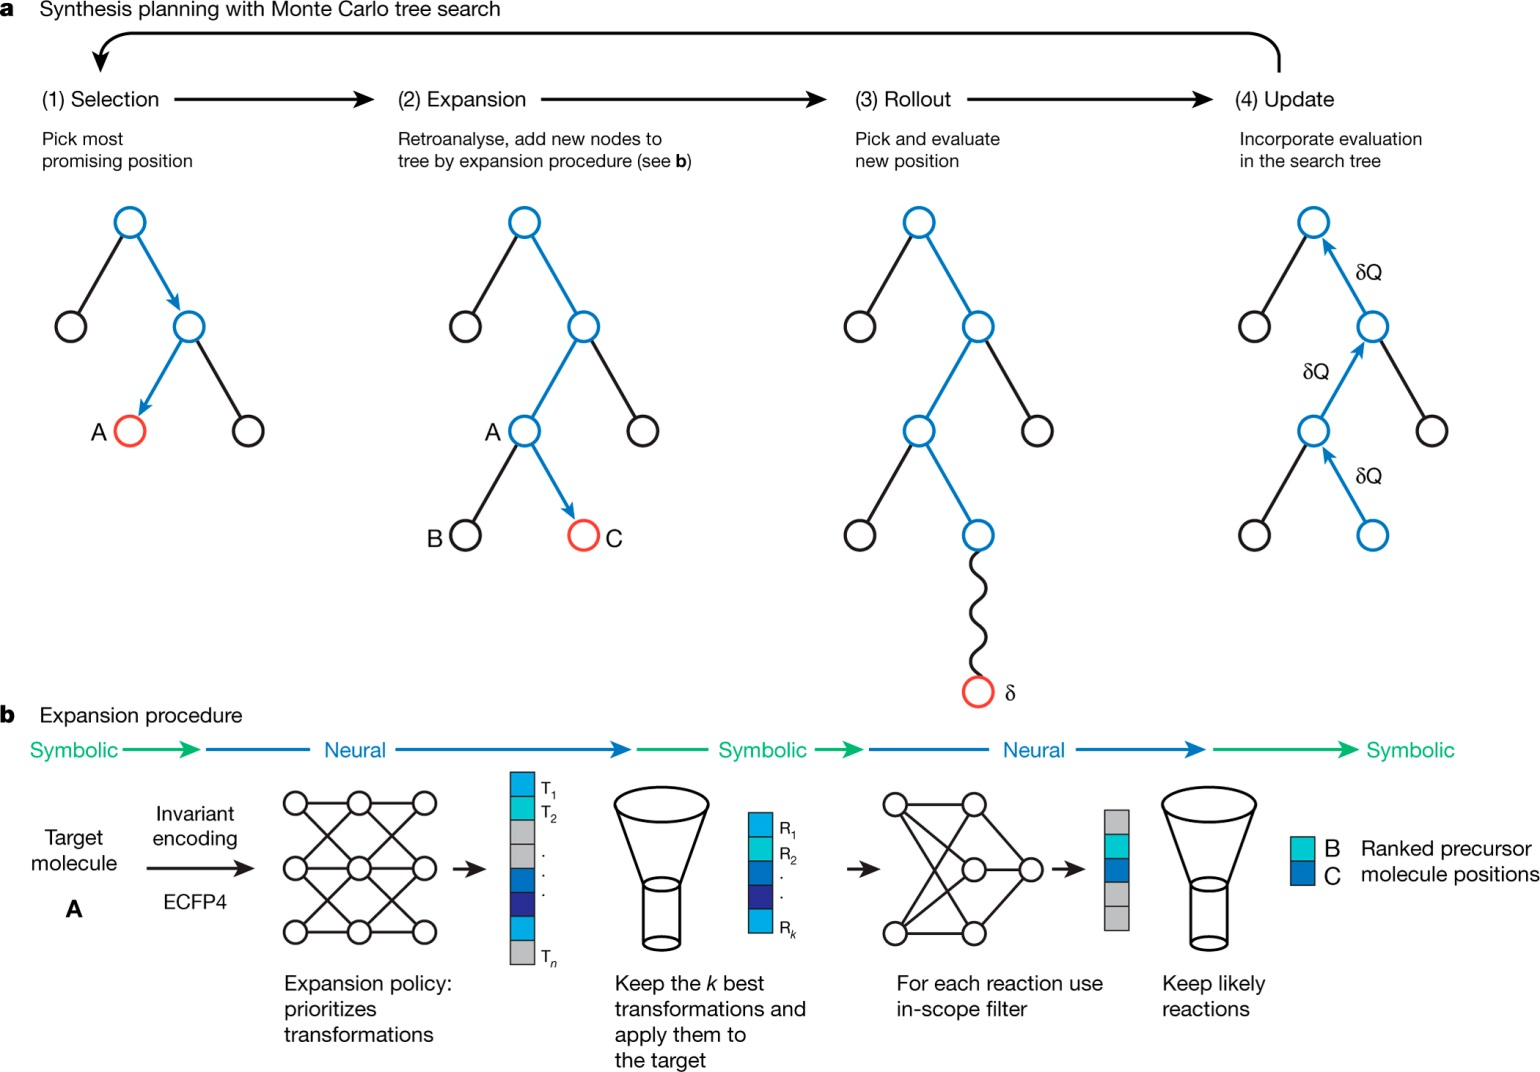
\includegraphics[width=\textwidth]{3N-MCTS-fig.jpg}
    \caption{3N-MCTS-mallin toimintaperiaate kuvattuna}
    {\cite{SeglerMarwinHS2018Pcsw}}
    {\label{fig:3n-mcts-model}}
\end{figure}

Saattaa kuitenkin olla, että synteesipolkua ei voida luoda.
Joko synteesipolun tutkimiseen menee liian kauan aikaa tai synteesipolku sisältää liian monta vaihetta yhdisteen syntetisoimiseen.


\subsubsection{EPN-verkko}

EPN-verkko muodostuu täysin kytketystä tasosta ja viidestä highway-tasosta.
Molemmissa tasoissa on käytetty aktivointifunktiona ELU-funktiota (Exponential Linear Unit).
Täysin kytketyssä tasossa suoritetaan dropout-toiminto, jonka jälkeen vain 30 prosenttia ensimmäisen tason solmujen tuloksista otetaan huomioon seuraavalla tasolla.
Dropout-toiminolla tarkoitetaan, että vain tietty osa kaikista edellisen tason palauttamista arvoista huomioidaan~\cite{hinton2012improving}.
Dropout-toiminto suoritetaan mallin koulutusvaiheessa ja pois jätettävät arvot valitaan sattumanvaraisesti.
Dropout-toiminnolla pyritään välttämään ylitulkintaa (Overfitting).
Tämän jälkeen jokaisen highway-tason jälkeen suoritetaan dropout-toiminto, jossa otetaan huomioon vain 10 prosenttia edellisen tason arvoista.
EPN-verkon viimeinen taso on softmax-taso, joka palauttaa todennäköisyysjakauman.
Tämä jakauma kertoo, kuinka todennäköisesti muunnossääntö \emph{a} muodostaa tuotteen \emph{m}.

\begin{figure}[!ht]
    \centering
    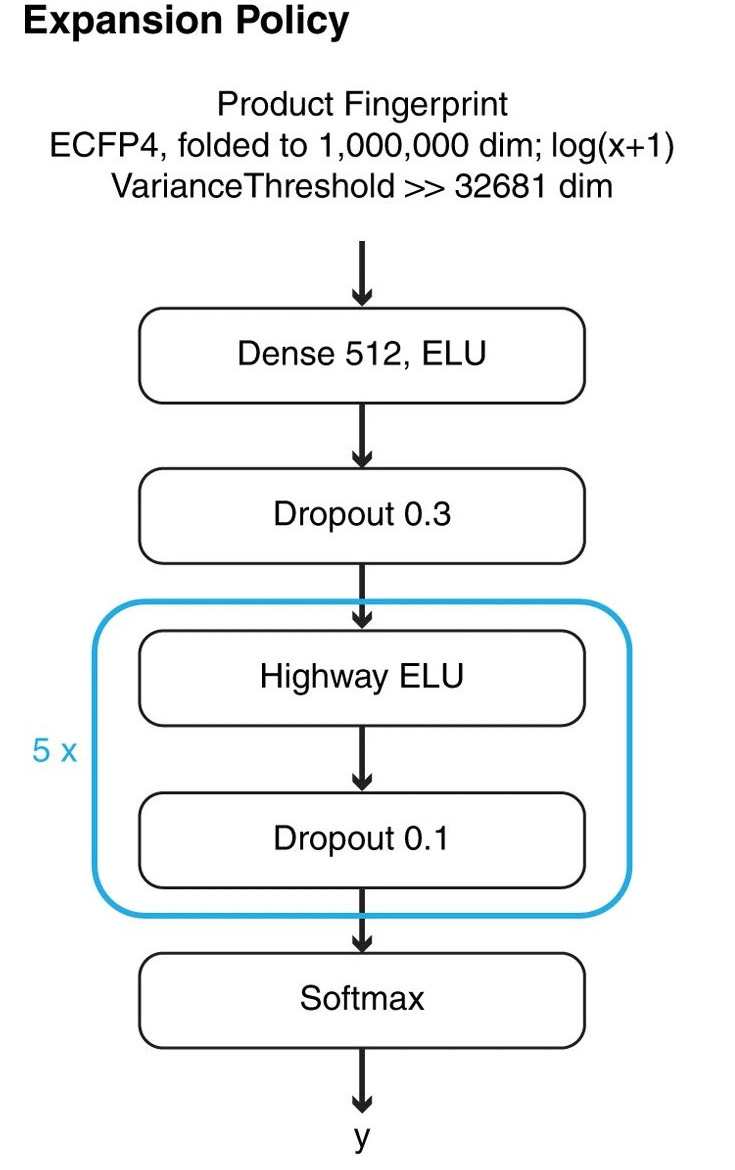
\includegraphics[]{expansion-policy.jpg}
    \caption{Kuvassa EPN-verkon rakenne.}
    {\cite{SeglerMarwinHS2018Pcsw}}
    {\label{fig:3n-mcts-epn}}
\end{figure}

EPN-verkon kouluttamiseen valittiin datasta vain reaktiokeskus.
Datasta suodatettiin pois sellaiset säännöt, jotka ilmenivät datassa alle kolme kertaa ennen vuotta 2015.
Lopullinen reaktiomäärä, jolla EPN-verkko koulutettiin, oli 301 671 reaktiota.

\subsubsection{RPN-verkko}

RPN-verkko muodostuu yhdestä täysin kytketystä tasosta.
Samalla tavalla kuin EPN-verkko, RPN-verkko käyttää myös ELU-funktiota aktivointifunktiona.
RPN-verkon ensimmäisen tason jälkeen suoritetaan dropout-toiminto, jonka jälkeen vain 40 prosenttia kaikista ensimmäisen tason arvoista tulkitaan.
RPN-verkon viimeinen taso on myös softmax-taso, joka palauttaa todennäköisyysjakauman.

\begin{figure}[!ht]
    \centering
    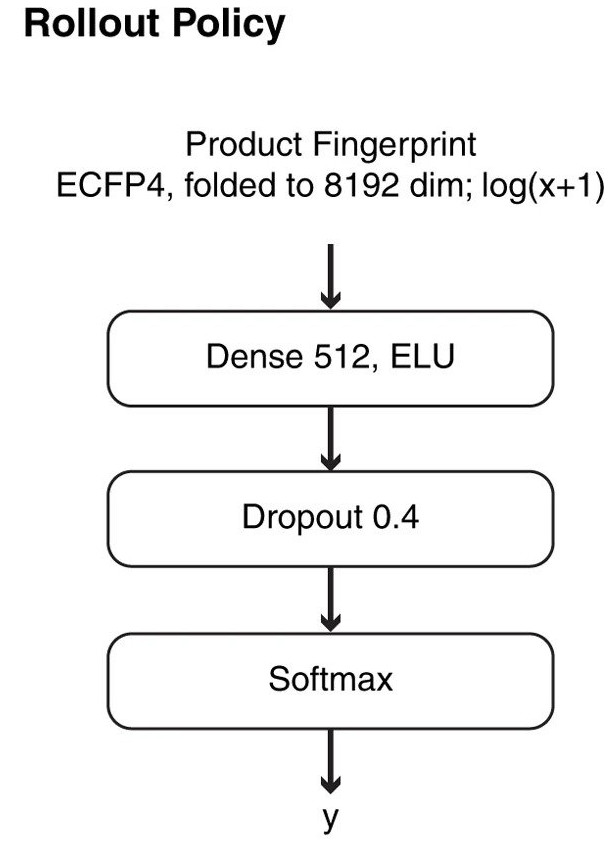
\includegraphics[]{rollout-policy.jpg}
    \caption{Kuvassa RPN-verkon rakenne.}
    {\cite{SeglerMarwinHS2018Pcsw}}
    {\label{fig:3n-mcts-rpn}}
\end{figure}

RPN-verkon kouluttamiseen valittiin datasta vain reaktiossa muuttuneet atomit ja liitokset (Reaktiokeskus) ja lähimmät vierekkäiset atomit.
Datasta suodatettiin pois sellaiset säännöt, jotka ilmaantuivat alle 50 kertaa ennen vuotta 2015.
Lopullinen reaktiomäärä, jolla RPN-verkko koulutetaan, on 17 134 reaktiota.

\subsubsection{IFN-verkko}

3N-MCTS-mallissa IFN-verkko toimii binääriluokittelijana.
IFN-verkko kertoo, onko sille annettu yhdiste mahdollista muodostaa annetulla muunnossäännöllä.

IFN-neuroverkko muodostuu kahdesta haarasta.
Toinen haara saa syötteenä muodostettavan yhdisteen tunnisteen ja toinen haara saa muunnossäännön tunnisteen.

Haara, joka saa syötteenä yhdisteen tunnisteen, muodostuu yhdestä täysin kytketystä tasosta jonka jälkeen suoritetaan 30 prosentin dropout-toiminto.
Tämän jälkeen data kulkee viiden highway-tason läpi.
Sekä täysin kytketty että highway-tasot käyttävät ELU-funktiota aktivointifunktiona.

Haara, joka saa syötteenä muunnossäännön tunnisteen, muodostuu vain yhdestä täysin kytketystä tasosta.
Tämä taso käyttää myös ELU-aktivointifuktiota.

Näiden haarojen jälkeen saaduista tuloksista lasketaan niiden kosinisamankaltaisuus.
Saatu tulos syötetään sigmoid-funktiolle, jonka tulos kertoo, pystyykö kyseinen muunnossäntö muodostamaan halutun yhdisteen.

\begin{figure}[!ht]
    \centering
    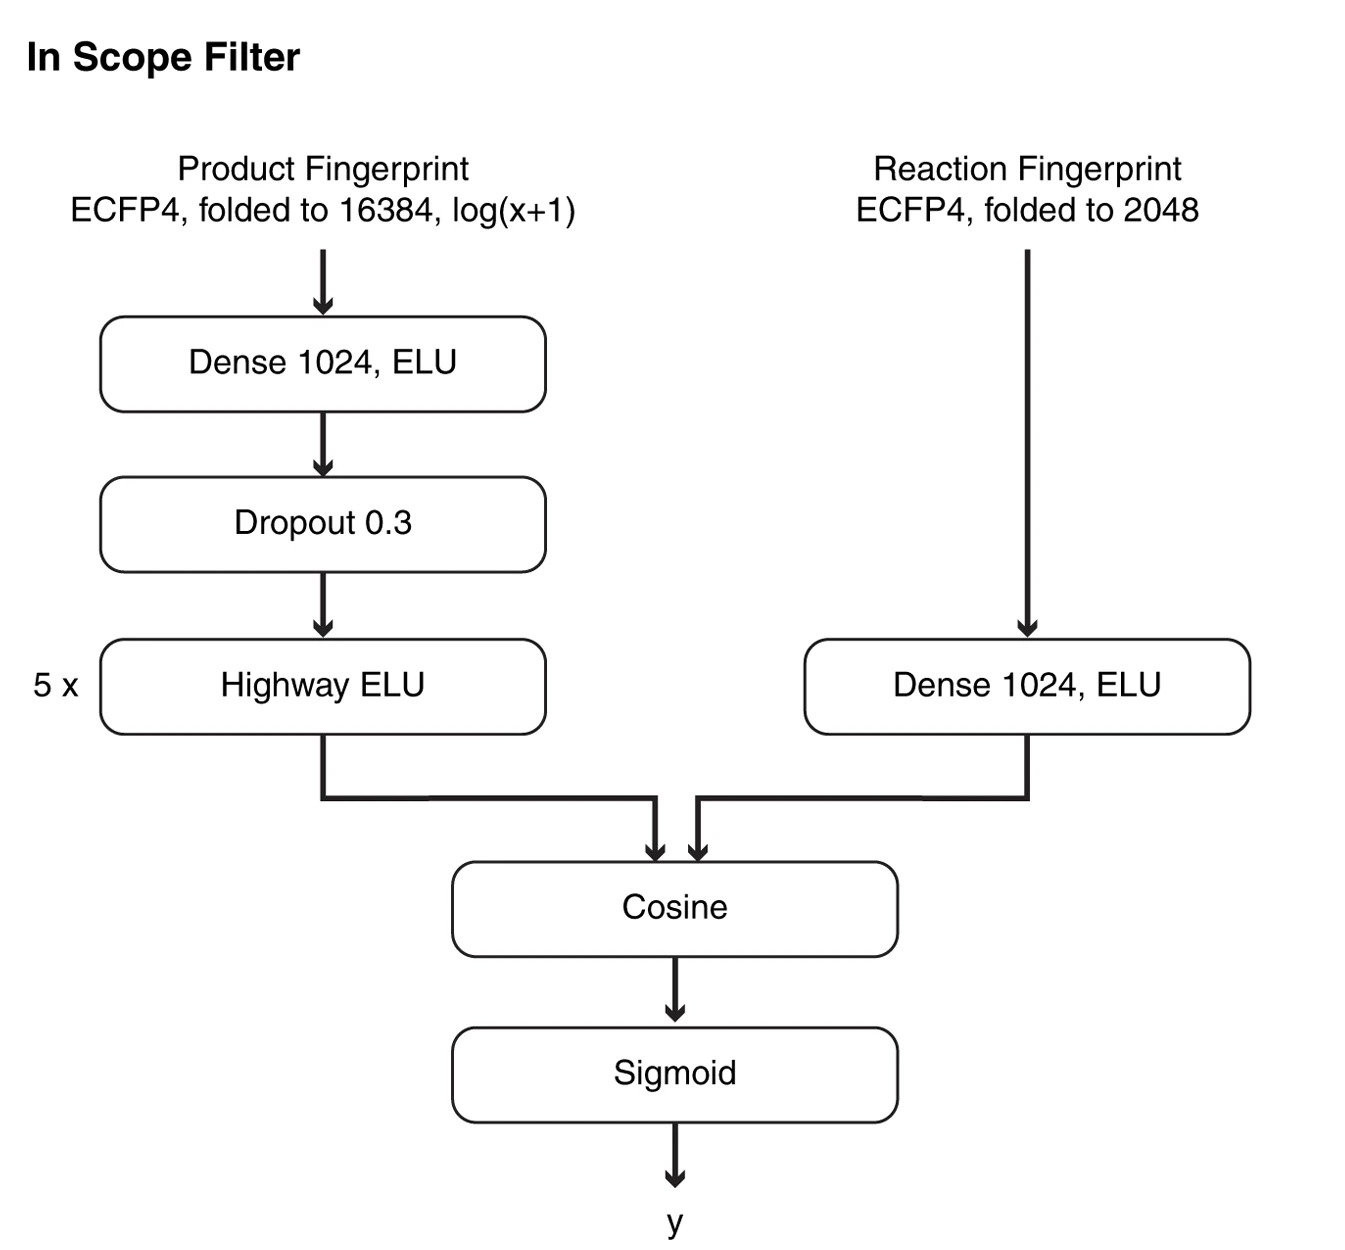
\includegraphics[]{in-scope-filter.jpg}
    \caption{Kuvassa IFN-verkon rakenne.}
    {\cite{SeglerMarwinHS2018Pcsw}}
    {\label{fig:3n-mcts-ifn}}
\end{figure}

IFN-verkko koulutetaan sekä onnistuneiden että epäonnistuiden sääntöjen avulla.
Koska epäonnistuneita sääntöjä ei tallenneta tietokantaan, niin kyseinen data generoidaan.
Data generoidaan niin, että jos reaktiossa \[A + B \rightarrow C\] lähtöaineet A ja B muodostavat reaktiossa lopputuotteen C, niin lopputuotteita D, E, F, jne.\ ei muodostu näistä.
IFN-verkon kouluttamista varten luotiin 100 miljoonaa epäonnistunutta reaktiota ja 10 miljoonaa epäonnistunutta reaktiota luotiin testaamista varten.

\subsubsection{3N-MCTS-mallin suorituskyky}

3N-MCTS-mallin suorituskykyä verrattiin BFS-menetelmään (Best-First Search -Method), joka käyttää heuristista käsin koodattua \(SMILES^{3/2}\)-kustannefunktiota.
Tämä funktio antaa parhaimman tuloksen muunnossäännölle, joka jakaa halutun yhdisteen mahdollisimman hyvin yhtä suuriin lähtötuotteisiin.
Tästä menetelmästä luotiin myös versio, joka käyttää muokattua \(SMILES^{3/2}\)-kustannefunktiota.
Muokattu funktio käyttää 3N-MCTS-mallin EPN- ja IFN-verkkoja parhaimman muunnossäänön selvittämiseksi.

Mallit koulutettiin samoilla muunnossäännöillä ja testeissä käytettiin samaa aikaan perustuvaa jakoa.
Mallit koulutettiin muunnossäännöillä, jotka ilmenivät ennen vuotta 2015, ja malleja testatiin vuoden 2015 jälkeen ilmenneillä muunnossäänöillä.

Mallien tehtäväksi annettiin löytää halutulle yhdisteelle retrosyntetisointipolku annetussa ajassa.
Testaamiseen käytettiin 497 eri yhdistettä.
Mittaukset on kuvattu kuvaajassa~\ref{fig:3n-mcts-performance}.

3N-MCTS-malli suoriutui kahta muuta menetelmää paremmin jokaisessa eri aikakategoriassa.
3N-MCTS-malli löysi viidessä sekunnissa 80 prosentille yhdisteistä retrosyntetisointipolun, kun taas muokattu \(SMILES^{3/2}\)-menetelmä löysi retrosyntetisointipolun vain 40 prosenttille yhdisteistä ja alkuperäinen ei löytänyt polkuja lainkaan.
Kun aikaa kasvatettiin 60 sekunttiin per yhdiste, 3N-MCTS-malli löysin 92 prosentille yhdisteistä polun, muokattu \(SMILES^{3/2}\) löysi 71 prosentille yhdisteistä ja alkuperäinen versio vain 4 prosentille yhdisteistä polun.

3N-MCTS-mallia testattiin myös sokkotestillä 45 yliopistotason kemistille.
Testin tarkoituksena oli selvittää, suosivatko henkilöt ennemmin kirjallisuuteen perustuvaa retrosyntetisointipolkua vai 3N-MCTS-mallin antamaa polkua.
Sokkotestissä 57 prosenttia henkilöistä valitsi 3N-MCTS-mallin muodostaman polun ja loput valitsivat kirjallisuuteen perustuvan polun.

\begin{figure}[!ht]
    \centering
    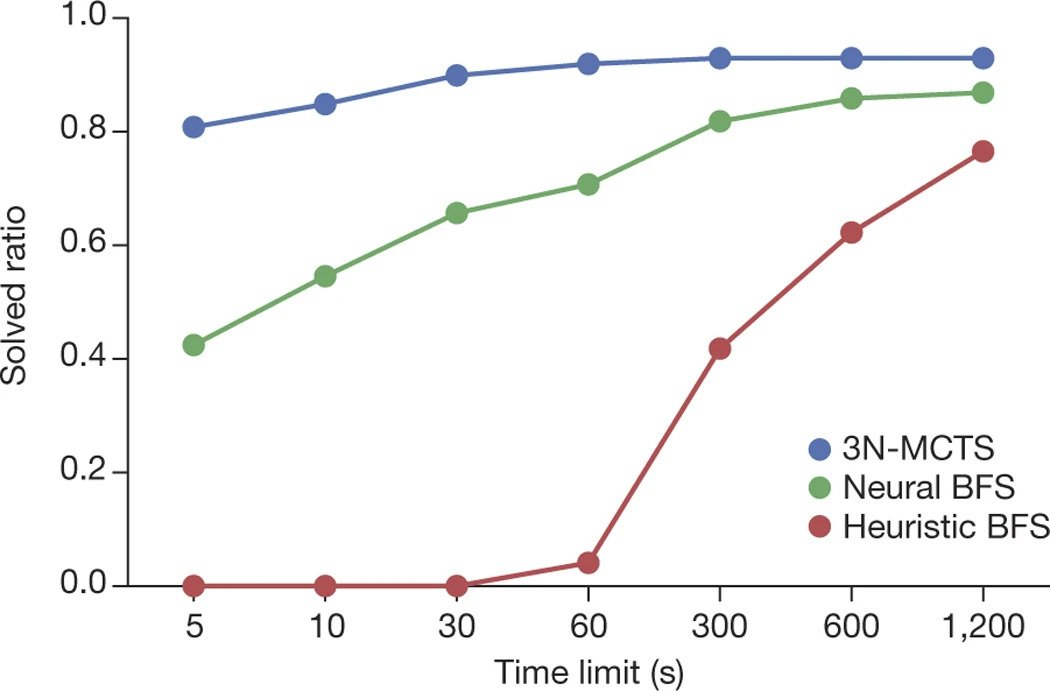
\includegraphics[width=8cm, height=6cm]{3N-MCTS-performance-fig.jpg}
    \caption{
        3N-MCTS-mallin suorituskyky verrattuna \(SMILES^{3/2}\)-menetelmään hyödyntävään BFS-menetelmään ja 3N-MCTS-mallin neuroverkkoja hyödyntävään BFS-menetelmään.
        Kuvaaja kertoo, kuinka monelle prosentille annetuista yhdisteistä menetelmä kykenee löytämään retrosyntetisointipolun annetusssa ajassa.
        Annetulla ajalla tarkoitetaan aikaa, jonka menetelmä voi korkeintaan käyttää yhden yhdisteen retrosyntetisointipolun löytämiseen.
    }
    {\cite{SeglerMarwinHS2018Pcsw}}
    {\label{fig:3n-mcts-performance}}
\end{figure}

\subsection{ICHO-malli}

On myös yleistä, että retrosynteesipolkuja suunnitelevat mallit hyödyntävät heurustiikkaa~\cite{ExpertKnowledgeRetorsynthesis}.
Badowski et al.\ ryhmä on kehittänyt koneoppimismallin, joka ehdottaa tietylle yhdisteelle parasta mahdollista muunnossääntöä, jonka avulla yhdiste voidaan muodostaa.
Kehitetty ICHO-malli hyödyntää  neuroverkkoja ja ammattikemistien muodostamia heuristisia sääntöjä pisteyttäessään muunnossääntöjä.
ICHO-malli on verrattavissa 3N-MCTS-mallin EPN- ja IFN-verkkojen toimintaan.

ICHO-mallin (Instytut Chemii Organicznej) kouluttamisessa käytettiin dataa 1.4 miljoonasta reaktiosta ja niiden lopputuotteista.
Data saadaan julkaistuista artikkeleista ja patenteista.
Reaktiolta kuitenkin vaaditaan, että ainakin yksi reaktio per lopputuote löytyy myös Chematican Expert-Coded säännöstöstä.
Datasta suodatettiin pois myös suojaryhmien säännöt.
Chematica on retrosyntetisointia suunnitteleva ohjelmisto ja tietokanta, joka sisältää dataa kemiallisista reaktioista~\cite{synthia}.
Chematican omistaa Merck KGaA inc.\ ja sen nimi nykyään on Synthia.

ICHO-mallista kehitettiin myös malli, jonka kouluttamisessa käytettiin lisäksi vektoreita, jotka sisälsivät dataa kemiallisesti intuitiivisistä reaktiopiirteistä, joita on käytetty aikaisemmissa tutkimuksissa.
Tätä mallia kutsutaan ICHO+ -malliksi, ja sitä käytetään vertailemaan ICHO-mallin suoriutumista.

Kehitetyssä ICHO-mallissa on kaksi tärkeää asiaa.

\begin{enumerate}
    \item Se laskee reaktioiden ilmaantumistodennäköisyyttä uudelleen perustaen kuinka usein ne ilmaantuvat ammattilaisten käyttämissä reaktioissa.
          Tämä laskenta tapahtuu mallin koulutusvaiheessa.
          Käytännössä tämä tarkoittaa, että koulutusvaiheessa mallilla on tieto, kuinka monta kertaa tietty reaktiosääntö ilmeni datassa ja kuinka monta kertaa kyseistä reaktiota käytettiin luomaan jokin lopputuote.
          Malli laskee näiden välisen suhteen, jolloin se pystyy määrittämään, kuinka usein kyseistä reaktiota kannattaa käyttää.
          Jos esimerkiksi reaktio on mainittu datassa kymmenen kertaa ja samassa datassa kyseistä reaktiota käytetään kymmenen kertaa luomaan jokin lopputuote, niin malli käyttää tätä reaktiota, koska se luokitellaan `Helpoksi ja varmaksi toteuttaa'.
          Jos suhde taas on pieni, niin reaktio luokitellaan `vaikeaksi toteuttaa'.

    \item Se kykenee antamaan suuremman kuin nollatodennäköisyyden reaktiolle, joka ei ilmaantunut koulutusvaiheessa.
          Tämä sen takia, että mallille koulutetaan jatkuva funktio, joka antaa todennäköisyyden jokaiselle reaktiotyypille perustuen, kuinka reaktio muuttaa lopputuotteen lähtötuotteiksi.
          Eli jos jokin reaktion sormenjälki tai heuristinen kuvaus on samankaltainen toisen reaktion kanssa, joka ilmenee koulutusdatassa, niin reaktiolle voidaan antaa todennäköisyys sen käytölle.
\end{enumerate}

\begin{figure}[!ht]
    \centering
    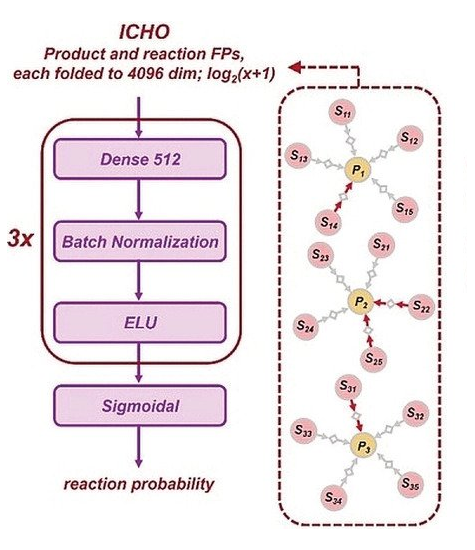
\includegraphics[width=8cm, height=8cm]{icho-neuralnetwork.png}
    \caption{ICHO-mallin rakenne.}
    {\cite{ExpertKnowledgeRetorsynthesis}}
    {\label{fig:icho-neuralnetwork}}
\end{figure}

ICHO-malli muodostuu neljästä tasosta, joista kolme tasoa ovat täysin kytkettyjä neuroverkkoja ja viimeinen taso on sigmoid-taso
Malli kuvattu kuvassa~\ref{fig:icho-neuralnetwork}.
Samalla tavalla kuin 3N-MCTS-mallissa, ICHO-malli käyttää myös ELU-aktivointifunktiota.
ICHO-malli käyttää Batch normaliztion -algoritmia koulutusvaiheessa.
Batch Normalization -algoritmin idea on standardoida koulutusvaiheessa tasolle tuleva syöte, jolla verkon painoja muutetaan.

ICHO-mallia vertailtiin aikasiemmin mainitun 3N-MCTS-mallin kanssa, jota kutsutaan artikkelissa SW-mallina.
Kyseisestä SW-mallista kehitettiin myös heuristista dataa hyödyntävä malli SW+.
Lisäksi luotiin SW-malli, joka ei käy läpi kaikkia mahdollisia reaktioita, vaan valitsee säännöt niistä reaktioista, jotka eivät aiheuta konfliktia ja jotka johtavat vain tiettyyn lopputuotteeseen.
Tätä mallia kutsutaan SW2-malliksi ja tästä luodusta heuristisesta mallista käytetään nimeä SW2+.
Lisäksi vertailumalliksi luodaan täysin heuristinen \(SMALLER\)-malli, joka arvioi reaktioita sen mukaan, kuinka paljon ne rakenteellisesti yksinkertaistavat lopputuotetta.
Tämä malli suosii reaktioita, jotka pilkkovat molekyylin keskeltä eli puolittavat sen.
Tämä on haluttu lähestymistapa retrosynteesiin, koska se minimoi syntetisointivaiheiden määrän.

\subsubsection{ICHO-mallin suorituskyky}

ICHO-mallia testataan eri tavalla kuin 3N-MCTS-mallia, jossa mitataan, kuinka monelle yhdisteelle malli kykenee löytämään toimivan retrosyntetisointipolun tietyssä ajassa.
ICHO-mallia testataan siten, että jokaiselle mallille annetaan yhdiste, ja malli antaa tulosteena listan muunnossäännöistä, jotka on asetettu paremmuusjärjestykseen niille annetun pisteytyksen mukaan.
Muunnossäänön pisteytys kertoo, kuinka paljon malli suosittelee käytettävän kyseistä muunnossääntöä.
Näistä muunnossäännöistä lasketaan, kuinka suuri osa niistä pohjautuu johonkin aikaisempaan muunnossääntöön, joka on esiintynyt kirjallisuudessa.
Mitä suurempi osa ehdotetuista muunnossäänöistä löytyy kirjallisuudesta, sitä paremmin malli toimii.

Kuvaajaan~\ref{fig:icho-performance} on piirretty vain eri mallien heuristiikkaa hyödyntävät versiot, koska ne pärjäsivät testeissä ei-heuristisia versioita paremmin.
Lisäksi kuvaajaan on piirretty \emph{SMALLER}-malli vertailuksi.

Nähdään, että ICHO+ -malli pisteyttää kirjallisuuteen perustuvat muunnossäännöt paremmin kuin muut mallit, vaikkakin eroavaisuudet ovat vähäiset.

Kuvaajan~\ref{fig:icho-performance} kuvaajista b) ja c) nähdään, että pienelläkin koulutusaineistolla ICHO+ -malli sijoittaa kirjallisuuden muunnossäännöt korkeammalle kuin muut mallit ja mitä enemmän koulutuaineistoa käytetään mallin kouluttamiseen sitä suurempi osa korkeimmin sijoitetuista muunnossäännöistä perustuvat kirjallisuuteen.
Mielenkiintoinen huomio, mikä kuvaajasta nähdään on, että \emph{SMALLER}-malli sijoittaa kirjallisuuteen perustuvat säännöt pienemmällä koulutusaineistolla korkeammalle kuin suuremmalla aineistomäärällä.
SW2+ -malli taas toimii päinvastaisesti.
Mitä enemmän koulutusaineistoa se saa, sitä korkeammalle se sijoittaa kirjallisuuteen perustuvat säännöt.

Kuvaajat d) ja e) eivät ole ristiriidassa kuvaajien a), b) ja c) kanssa.
Kuvaajasta d nähdään, että nopeasti koulutusaineiston kasvaessa tutkittvat muunnossäännöt siirtyvät nopeasti korkeille sijoille SW2+ -mallissa ja ICHO+ -malli sijoittaa ne korkealle jo pienellä datamäärällä.
\emph{SMALLER}-malli sen sijaan sijoittaa tutkittavat muunnossäännöt koulutusaineiston kasvaessa huonommalle sijalle.
Kuvaaja e) myös näyttää, että ICHO+ -ja SW2+ -mallien MRR-pisteet (Mean Reciprocal Rank) kasvavat koulutusaineiston kasvaessa, kun taas \emph{SMALLER}-mallin pisteytys laskee.
MRR-pisteytyksellä tarkoitetaan kaikkien yhdisteiden sijoitusten käänteislukujen keskiarvoa.
Tällöin kuvaajan arvo lähestyy arvoa yksi, jos malli sijoittaa kaikki tutkittavat muunnossäännöt korkeille sijoille.

\begin{figure}[!ht]
    \centering
    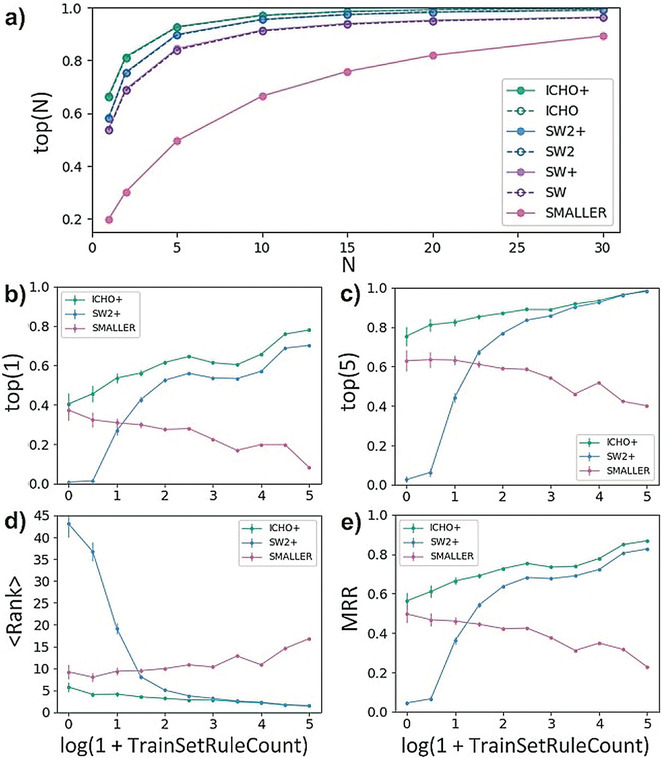
\includegraphics[width=10cm, height=10cm]{icho-performance-fig.jpg}
    \caption{
        ICHO-mallin ja muiden testattujen koneoppimismallien suorituskyky kuvattuna.
        Kuvaajat a-c kertovat, kuinka suuri osa n-määrästä parhaiten pisteytettyjä muunnossääntöjä oli jostain kirjallisuudesta, esim.\ raportti.
        Esimerkiksi top 1 = 1 tarkoittaa, että malli antaa parhaimman pisteytyksen aina kirjallisuuteen perustuvalle muunnossäännölle.
        Kuvaaja d kertoo, mille sijalle kukin malli sijoittaa tietyn muunnossäännön.
        Tässä tapauksessa rank = 1 tarkoittaa, että malli sijoittaa tietyn muunnossäännön aina sijalle yksi.
        Kuvaaja e kertoo keskiarvon kirjallisuuteen perustuvien muunnossääntöjen käänteisestä sijoituksesta.
        Tämä tarkoittaa, että jos malli sijoittaa kaikkien kirjallisuuteen perustuvat muunnossäännöt ensimmäiseksi, niin MRR saa arvon yksi.
    }
    {\cite{ExpertKnowledgeRetorsynthesis}}
    {\label{fig:icho-performance}}
\end{figure}

\chapter{Yhteenveto}

Tässä tutkielmassa avattiin yleisiä asioita, mitkä liittyvät uusien lääkkeiden löytämiseen, syntetisointisuunnitteluun ja kuinka koneoppimista voidaan hyödyntää näissä vaiheissa.
Lisäksi tutkielmassa käytiin läpi kolmen eri koneoppimismallin toimintaa ja niihin liittyviä asioita.

Johdannossa kerrottiin, mitä vaiheita kuuluu lääkekehitykseen ja miksi koneoppimista halutaan käyttää osana lääkekehityksen prosessia.
Tämä asettaa ongelman, miksi koneoppimista halutaan käyttää lääkekehityksen prosesseissa.
Vaikka käyttökohteita koneoppimiselle on jokaisessa lääkekehityksen vaiheessa, niin tutkielmassa keskityttiin vain lääkkeiden löytämiseen ja lääkkeiden syntetisointisuunnitteluun koneoppimismenetelmillä.
Nämä käytiin läpi sen takia, koska ne ovat kliinisten testien jälkeen vaiheet, joihin kuluu eniten resursseja.
Nämä käytiin läpi myös sen takia, koska ongelmat ja konseptit, joita lääkkeiden löytämisessä ja syntetisoinninsuunnittelussa käytiin läpi, on suhteellisen helppoja ymmärtää ilman syvällisempää kemiaan tai lääkkeisiin liittyvää tietoa.
Tämän takia tutkielma pystyi keskittymään enemmän kehitettyihin koneoppimismalleihin ja niiden taustoihin.

Johdannon jälkeen kerrottiin, mitä eri datatyyppejä käytetään tutkielmassa käytävien koneoppimismallien kouluttamisessa.
Tämän kappaleen sisällön avaaminen auttaa ymmärtämään koneoppimismallien toimintaa ja mitä ongelmia ne ratkovat.

Kappaleessa kolme keskityttiin lääkkeiden löytämiseen ja sen taustoihin.
Tätä aihetta avattiin tutkielmassa, koska sen nopeuttaminen ja tehostaminen mahdollistaa haluttujen ominaisuksien omaavien lääkkeiden nopean löytämisen.
Jos koneoppimismallit pystyvät luomaan sellaisia yhdisteitä kuvaavia merkkijonoja, joilla on tarkkaan määritellyt ominaisuudet, niin tarve ja tarvittava aika lääkeyhdisteiden ominaisuuksien jatkotutkimukselle vähenee.
Kappaleessa avattiin yhden toteutetun koneoppimismallin toimintaa, joka luo uusia yhdistemerkkijonoja haluttujen ominaisuuksien perusteella.
Tämä antoi hieman ajatusta, millä tavalla uusia yhdisteitä voidaan etsiä ja mitä asioita liittyy lääkkeiden etsimiseen.

Kappaleessa neljä käytiin läpi, mitä asioita liittyy yhdisteiden syntetisointisuunnitteluun.
Tätä aihetta avattiin tutkielmassa sen takia, koska syntetisointisuunnittelu on osa lääkkeiden löytämis- ja kehitysvaihetta, ja tämän aiheen tutkiminen voi luoda uusia ja tehokkaampia tapoja, kuinka syntetisointia voidaan toteutaa käytännössä.
Vaikka tutkielmassa keskityttiin syntetisointisuunnitteluun lääkkekehityksen näkökulmasta, niin syntetisointisuunnittelua voidaan tehostaa koneoppimismenetelmillä kaikessa materiaalitieteissä niin kauan, kun aiheeseen liittyvää dataa on saatavilla.

Kappaleessa neljä avattiin myös kahden eri koneoppimismallin toimintaa.
Ensimmäinen malli, 3N-MCTS, on kokonaisempi malli, joka palauttaa yhdisteen syntetisointipolun.
Tämän mallin avaaminen antaa ajatusta, kuinka puuhaku- tai reitinhakualgoritmeja voidaan käyttää syntetisointipolkujen etsimisessä ja kuinka neuroverkot toimivat niiden tukena.
Mallin toimintaperiaatteen avaaminen myös näyttää, kuinka raakaa reaktiodataa voidaan käyttää syntetisoinninsuunnittelussa.
Toinen malli, ICHO, taas puolestaan palauttaa parhaimman muunnossäännön, jonka avulla yhdiste voidaan luoda.
Se ei etsi syntetisointireittejä, mutta se käyttää heuristiikka apunaan muunnossääntöjen etsimisessä.
Näiden mallien avaaamisen tarkoituksena on näyttää, että syntetisointisuunnittelua voidaan suorittaa usealla tavalla ja kuinka eri tapojen suorituskykyä voidaan verrata toisiinsa.

Lääkekehitys on pitkä ja kallis prosessi, ja koneoppimismenetelmillä on mahdollisuus vähentää siihen kuluvaa aikaa ja rahaa.
Tutkielmassa avatuilla koneoppimismalleilla ja useilla muilla kehitetyillä malleilla voidaan tehostaa lääkekehityksen vaiheita.
Tutkimusta tehdään tällä tutkimusalueella paljon ja uusia malleja kehitetään jatkuvasti.
Tutkimuksen ja kehitettyjen koneoppimismallien määrä näyttääkin viittaavaan, että tulevaisuudessa koneoppiminen tulee olemaan merkittävä osa lääkekehitystä.

\cleardoublepage{}                          %fixes the position of bibliography in bookmarks
\phantomsection{}
\addcontentsline{toc}{chapter}{\bibname}  % This lines adds the bibliography to the ToC
\printbibliography{}

%%%%%%%%%%%%%%%%%%%%%%%%%%%%%%%%%%%%%%%%%%%%%%%%%%%%%%%%%
\backmatter{}
% \begin{appendices}

%     \appendix{Sample Appendix\label{appendix:model}}
%     usually starts on its own page, with the name and number of the appendix at the top.
%     The appendices here are just models of the table of contents and the presentation. Each appendix
%     Each appendix is paginated separately.

%     In addition to complementing the main document, each appendix is also its own, independent entity.
%     This means that an appendix cannot be just an image or a piece of programming, but the appendix must explain its contents and meaning.

% \end{appendices}
%%%%%%%%%%%%%%%%%%%%%%%%%%%%%%%%%%%%%%%%%%%%%%%%%%%%%%%%%

\end{document}
